\documentclass{article}
\usepackage{graphicx}
\usepackage{caption}
\usepackage{subcaption}
\usepackage{subfig}

\begin{document}


\section{The Eclipse ICE Developer Menu}

\subsection{Overview}
The Eclipse Integrated Computational Environment (ICE) has had a great track
record of providing a comprehensive environment for general scientific
computing. Tasks such as model input generation, local and remote simulation
execution, and post-simulation data analysis and visualization are all very well
supported in the application. This takes care of the majority of needs for
\emph{using} general scientific computing codes, but what about
\emph{developing} those applications to begin with? Is there 
any way ICE can be extended to provide
support for the development of science codes? 

\begin{center}

\includegraphics[width=12cm]{figures/icemenu.png}
\label{fig:devmenu}
\end{center}

The answer is yes! In 2015 ICE was extended to provide support for scientific
application \emph{development} through a custom, extensible \textbf{Developer} 
top-level menu. This menu is shown in Figure
\ref{fig:devmenu} and provides custom actions that enable efficient scientific
application development for both novice and expert users of a given science
code.

The Developer Menu is completely customizable through Eclipse Extension Points.
Specifically, ICE exposes a new extension point:
\emph{org.eclipse.ice.developer.code}. This extension point provides the means
to specify details about a scientific code: its name, category (Framework,
Nuclear, Other, etc\ldots), and where its repository is hosted, just to name a
few. This point also enables the addition of \emph{commands} that point to some
custom subclass of \emph{org.eclipse.core.commands.AbstractHandler} that
performs some task related to the development of the code. 

With these extension points exposed as part of an ICE product execution, ICE
handles all the complexity of picking them up and populating the Developer Menu
dynamically at runtime. This is be shown in Figure \ref{fig:devcloneice}, with
an ICE category for ICE development, and another for scientific frameworks. This
is exactly how ICE developers work on ICE itself - by pulling down the ICE
binary and leveraging the Developer Menu to clone and build ICE, all within ICE.
ICE also provides these hooks for other scientific codes, like the Multiphysics
Object Oriented Simulation Environment (MOOSE) for general finite-element
simulations. ICE provides a hook for cloning MOOSE and for forking a templated
repository for MOOSE Application development.

\begin{center}
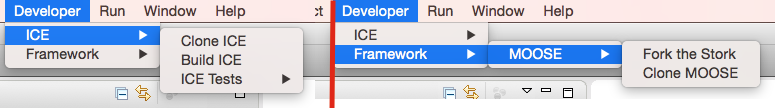
\includegraphics[width=\textwidth]{figures/menu.png}
\label{fig:devcloneice}
\end{center}

Extending the Developer Menu is easy, and relies on simply creating a new plugin
and exposing a new extension point. Let's see how to do this in detail:

\subsection{Extending the ICE Developer Menu}
\subsubsection{Create a New Plugin Project}
\subsubsection{Create a New ICE Developer Extension Point}
\subsubsection{Setup ICE to Run with the New Plugin}

\end{document}
